\chapter{Grundlagen zu planaren Graphen}\label{prerequisites}

Planare Graphen haben, durch die Existenz kreuzungsfreier Einbettungen, in gewissem Sinne besonders schöne Zeichnungen und so ist einer der Fragen mit der sich schon viele Mathematiker auseinander gesetzt haben: \textit{"How to draw a Graph?"}\cite{tutte63}\\

Bei topologische Zeichnung eines planaren Graphen werden die Kanten als Kurven dargestellt die sich nur in den Knoten treffen. In den Fünfzigern wurde unter anderem von István Fáry gezeigt, dass für jeden planaren Graphen mit einem beliebigen äusseren Gebiet eine geradlinige Zeichnung existiert. \cite{fary48}

\begin{figure}
	\centering
  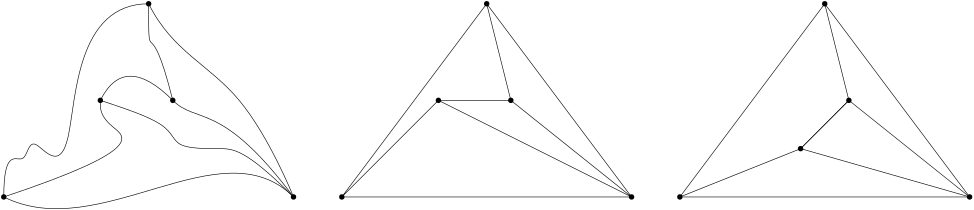
\includegraphics[width=0.9\textwidth]{topo_straight_convex.png}
	\caption{Planarer Graph mit einer topologischen, einer geradlinigen und einer konvexen Zeichnung.}
	\label{cut_figure}
\end{figure}

\begin{definition}[intern zusammenhängend]\label{int_3_con}
Ein Graph $G$ ist zusammenhängen falls für alle Knoten $u,v$ ein Pfad von $u$ nach $v$ exisitert. $G$ ist \textit{k-zusammenhängend}, falls er nach der Entfernung von $k-1$ beliebigen Knoten weiterhin zusammanhängend ist.\\
Sei $G$ plan mit den Aufhängungen $a_1,s_2,a_3$, weiter sei $a_\infty$ ein zusätzlicher Knoten im äusseren Gebiet. Dann ist $G$ \textit{intern k-zusammenhängend}, falls $G \cup \{ a_1a_\infty,a_2a_\infty,a_as_\infty \}$ k-zusammenhängend ist. 
\end{definition}

In den Siebzigern betrachtete William Thomas Tutte die Unterklasse der drei-zusammenhängenden planaren Graphen und zeigte, dass für diese nicht nur geradlinige, sondern sogar \textit{konvexe} Zeichnungen existieren, bei denen alle Gebiete die konvexe Polygone umranden. \cite{tutte63}

\section{Geradlinige Dreiecks Darstellungen (SLTRs)}

Ausgehend von der konvexen Darstellung nach Tutte, kann man sich die Frage stellen unter welchen Vorraussetzungen wir einen planaren Graphen so zeichnen können, dass alle Gebiete, inklusive dem Äusseren Dreiecken umranden. Bei der Formalisierung dieser Darstellung und ersten Feststellungen halten wir uns an Nieke Aerts und Stefan Felsner \cite{af13}.

\begin{definition}[SLTR]\label{defsltr}
Eine Zeichnung eines planen Graphen $G$ wird Gradlinige Dreiecks Darstellung, im weiteren kurz \textit{SLTR} (für die englische Bezeichnung Staight Line Triangle Representation), genannt falls gilt:
\begin{itemize}
\item[S1] Alle Kanten Segmente von Geraden
\item[S2] Alle Gebiete, inklusive dem äusseren, sind nicht degenerierte Dreiecke.
\end{itemize}
\end{definition}

\begin{figure}[h]
	\centering
  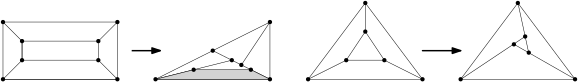
\includegraphics[width=0.9\textwidth]{sltr-example.png}
	\caption{Links einer der beiden drei-zusammenhängenden Graphen auf acht Knoten ohne SLTR und rechts ein Graph mit einer möglichen SLTR.}
\end{figure}

Um die Problemstellung greifbarer zu machen werden wir planare Graphen zusammen mit den drei Aufhängungen $a_1,a_2$ und $a_3$ als designierten Ecken einer möglichen SLTR betrachten. Einen Graphen zusammen mit einem äusseren Gebiet bzw. Aufhängungen zu betrachten, macht auch in sofern Sinn, dass kombinatorische Graphen existieren, von denen manche Einbettungen SLTRs zulassen, andere jedoch nicht, so wie in Abbildung \ref{10_example} zu sehen.

\begin{figure}
	\centering
  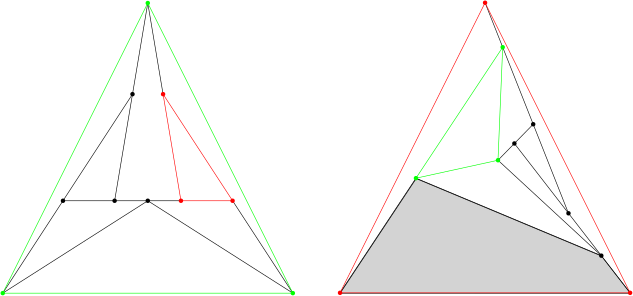
\includegraphics[scale=0.1]{10_example.png}
	\caption{Der kleinste drei-zusammenhängende Graph mit einer einer SLTR Einbettung und einer Auswahl der Aufhängung die kein SLTR zulässt.}
	\label{10_example}
\end{figure}

\begin{proposition}
Sei $G$ ein Graph mit Aufhängungen $a_1,a_2,a_3$ als äusseren Ecken einer SLTR. Weiter gebe es keinen Knoten von Grad zwei der in beiden angrenzenden Gebieten den Winkel $\pi$ hat\footnote{Ein solcher Knoten ist keine Aufhängung, da der Aussenwinkel grösser als $\pi$ ist. Alle anderen Knoten haben $\leq\pi$ Winkel. Somit können wir ihn durch eine gerade Kante zwischen seinen Nachbarn ersetzen und den resultierenden Graphen betrachten.}. Dann ist $G$ intern-drei-zusammenhängend\ref{int_3_con}.
\end{proposition}

%% TODO do i want the Proof??

Wir werden also von nun an, der Einfachheit halber intern-drei-zusammenhängende Graphen mit Aufhängungen betrachten, da alle anderen Graphen mit SLTR auf diese reduziert werden können. \\

Zu den Fragen, welche notwendigen und hinreichenden Bedingungen es für die Existenz von SLTRs gibt und  welche algorithmischen Ansätze es bei der Suche nach einer spezifischen Darstellung gibt haben Aerts und Felsner in \cite{af13}, \cite{af13h} und \cite{af15} schon einige Antworten geliefert, mit denen wir uns in den nächsten beidem Kapiteln beschäftigen werden. Zuerst müssen aber in diesem Kapitel noch ein paar notwendige Konzepte eingeführt werden.


\section{Schnyder Wälder}\label{sw}
Schnyder Wälder, im weiteren \textit{Schnyder Woods} wurden zuerst von Walter Schnyder zur Betrachung der Ordungs-Dimension planarer Graphen, als eine Färbung und Orientierung auf den inneren Kanten einer Triangulierung, betrachtet \cite{schnyder89}. In einem weiteren Resultat dienten sie zur Erlangung einer planaren Einbettung auf einem $n-2 \times n-2$ Netz\cite{schnyder90}. Im Folgenden werden wir die Verallgemeinerung auf drei-zusammenhängende plane Graphen durch Felsner \cite{felsner01} und die zu ihnen in Bijektion stehenden Schnyder Labelings einführen.\\
\begin{definition}[Schnyder Woods]
Ein Schnyder Wood ist eine Orientierung und Beschriftung der Kanten von $G$ mit den Labeln 1, 2 und 3 unter Berücksichtigung der folgenden Regeln\footnote{Alternativ kann hier auch anschaulicher einfach von rot, blau und grün gesprochen werden. Es wird davon ausgegangen, dass die Label zyklisch sortiert sind, sodass $i+1$ und $i-1$ immer definiert sind.}:
\begin{itemize}
\item[W1] Jede Kante ist entweder un- oder bigerichtet. Falls sie bigerichtet ist haben beide Richtungen unterschiedliche Label.
\item[W2] An jeder Aufhängung  $s_i$ exisitert eine nach ausssen gerichtete Kante ohne Endpunkt mit Label i.  
\item[W3] Jeder Knoten $v$ hat hat Ausgangsgrad eins zu jedem Label. Um $v$ existieren im Uhrzeigersinn eine Auskante mit Label 1, null oder mehr eingehende Kanten mit Label 3, eine Auskante mit Label 2, null oder mehr  eingehende Kanten mit Label 1, eine Auskante mit Label 2 und null oder mehr  eingehende Kanten mit Label 2.
\item[W4] Es existiert kein gerichteter Zykel mit einem Label.
\end{itemize}

\end{definition}

\begin{figure}[h]
	\centering
  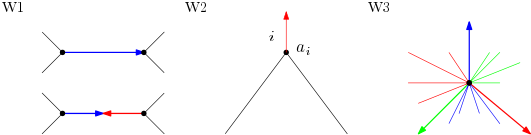
\includegraphics[width=0.9\textwidth]{schnyder_wood_def.png}
	\label{10_example}
\end{figure}

\begin{definition}[Schnyder Labeling]
Ein Schnyder Labeling ist eine Beschriftung Winkel von $G$ mit den Labeln 1, 2 und 3 unter Berücksichtigung der folgenden Regeln:
\begin{itemize}
\item[L1] Um jedes innere Gebiet bilden die Label im Uhrzeigersinn nichtleere Intervalle von 1en, 2en und 3en. Am äusseren Gebiet gilt dies gegen den Uhrzeigersinn.
\item[L2] An Aufhängung $a_i$ haben äusseren Winkel die Label i-1 und i+1 im Uhrzeigersinn mit der halben Auskante dazwischen und die inneren Winkel das Label i.\\
Um jeden inneren Knoten bilden die Label im Uhrzeigersinn nichtleere Intervalle von 1en, 2en und 3en.
\end{itemize} 

\end{definition}

\begin{theorem}
Schnyder Woods und Schnyder Labelings stehen in Bijektion zueinander.
// TODO  
\end{theorem}

// TODOBILD

\
